\subsection{Esercizio 22}
Tabulare il massimo errore di approssimazione (stimato su 10001 punti equidistanti
in $[0, 1]$) ottenuto approssimando le funzioni
\[
    \begin{array}{ccccc}
        sin(2\Pi x) & & e & & cos(2\Pi x)
    \end{array}
\]
mediante le function $spline0$ e $spline$, interpolanti su $n + 1$ punti equidistanti in $[0, 1]$,
per $n = 5, 10, 15, 20, \dots, 50$. Commentare i risultati ottenuti.
\newline \textbf{Soluzione:} \newline
% Sappiamo che $k = (b-a)$ e $k_n=(b-a)\frac{1}{n}\sum_{i=0}^{n}\abs{c_{in}}$. Il rapporto sarà dunque dato da: \[\dfrac{k_n}{k} = 
% \dfrac{(b-a)\frac{1}{n}\sum_{i=0}^{n}\abs{c_{in}}}{b-a} = \frac{1}{n}\sum_{i=0}^{n}\abs{c_{in}} \]
% Calcolando $\dfrac{k_n}{k}$ per $n = 1,.....,50$(\nameref{cod:22}) si ottiene:\\\\
%     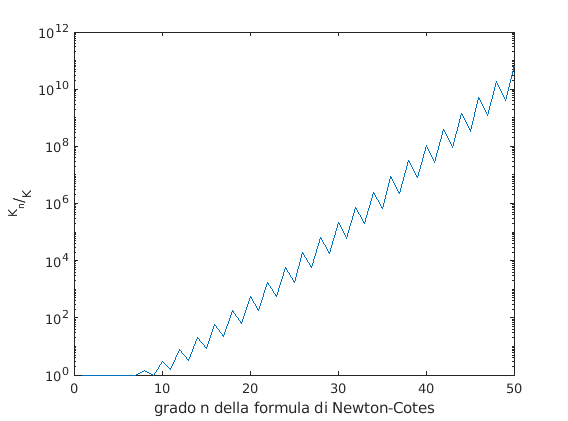
\includegraphics[width=\linewidth]{capitolo5/ncotes.png}

